\documentclass[1p]{elsarticle_modified}
%\bibliographystyle{elsarticle-num}

%\usepackage[colorlinks]{hyperref}
%\usepackage{abbrmath_seonhwa} %\Abb, \Ascr, \Acal ,\Abf, \Afrak
\usepackage{amsfonts}
\usepackage{amssymb}
\usepackage{amsmath}
\usepackage{amsthm}
\usepackage{scalefnt}
\usepackage{amsbsy}
\usepackage{kotex}
\usepackage{caption}
\usepackage{subfig}
\usepackage{color}
\usepackage{graphicx}
\usepackage{xcolor} %% white, black, red, green, blue, cyan, magenta, yellow
\usepackage{float}
\usepackage{setspace}
\usepackage{hyperref}

\usepackage{tikz}
\usetikzlibrary{arrows}

\usepackage{multirow}
\usepackage{array} % fixed length table
\usepackage{hhline}

%%%%%%%%%%%%%%%%%%%%%
\makeatletter
\renewcommand*\env@matrix[1][\arraystretch]{%
	\edef\arraystretch{#1}%
	\hskip -\arraycolsep
	\let\@ifnextchar\new@ifnextchar
	\array{*\c@MaxMatrixCols c}}
\makeatother %https://tex.stackexchange.com/questions/14071/how-can-i-increase-the-line-spacing-in-a-matrix
%%%%%%%%%%%%%%%

\usepackage[normalem]{ulem}

\newcommand{\msout}[1]{\ifmmode\text{\sout{\ensuremath{#1}}}\else\sout{#1}\fi}
%SOURCE: \msout is \stkout macro in https://tex.stackexchange.com/questions/20609/strikeout-in-math-mode

\newcommand{\cancel}[1]{
	\ifmmode
	{\color{red}\msout{#1}}
	\else
	{\color{red}\sout{#1}}
	\fi
}

\newcommand{\add}[1]{
	{\color{blue}\uwave{#1}}
}

\newcommand{\replace}[2]{
	\ifmmode
	{\color{red}\msout{#1}}{\color{blue}\uwave{#2}}
	\else
	{\color{red}\sout{#1}}{\color{blue}\uwave{#2}}
	\fi
}

\newcommand{\Sol}{\mathcal{S}} %segment
\newcommand{\D}{D} %diagram
\newcommand{\A}{\mathcal{A}} %arc


%%%%%%%%%%%%%%%%%%%%%%%%%%%%%5 test

\def\sl{\operatorname{\textup{SL}}(2,\Cbb)}
\def\psl{\operatorname{\textup{PSL}}(2,\Cbb)}
\def\quan{\mkern 1mu \triangleright \mkern 1mu}

\theoremstyle{definition}
\newtheorem{thm}{Theorem}[section]
\newtheorem{prop}[thm]{Proposition}
\newtheorem{lem}[thm]{Lemma}
\newtheorem{ques}[thm]{Question}
\newtheorem{cor}[thm]{Corollary}
\newtheorem{defn}[thm]{Definition}
\newtheorem{exam}[thm]{Example}
\newtheorem{rmk}[thm]{Remark}
\newtheorem{alg}[thm]{Algorithm}

\newcommand{\I}{\sqrt{-1}}
\begin{document}

%\begin{frontmatter}
%
%\title{Boundary parabolic representations of knots up to 8 crossings}
%
%%% Group authors per affiliation:
%\author{Yunhi Cho} 
%\address{Department of Mathematics, University of Seoul, Seoul, Korea}
%\ead{yhcho@uos.ac.kr}
%
%
%\author{Seonhwa Kim} %\fnref{s_kim}}
%\address{Center for Geometry and Physics, Institute for Basic Science, Pohang, 37673, Korea}
%\ead{ryeona17@ibs.re.kr}
%
%\author{Hyuk Kim}
%\address{Department of Mathematical Sciences, Seoul National University, Seoul 08826, Korea}
%\ead{hyukkim@snu.ac.kr}
%
%\author{Seokbeom Yoon}
%\address{Department of Mathematical Sciences, Seoul National University, Seoul, 08826,  Korea}
%\ead{sbyoon15@snu.ac.kr}
%
%\begin{abstract}
%We find all boundary parabolic representation of knots up to 8 crossings.
%
%\end{abstract}
%\begin{keyword}
%    \MSC[2010] 57M25 
%\end{keyword}
%
%\end{frontmatter}

%\linenumbers
%\tableofcontents
%
\newcommand\colored[1]{\textcolor{white}{\rule[-0.35ex]{0.8em}{1.4ex}}\kern-0.8em\color{red} #1}%
%\newcommand\colored[1]{\textcolor{white}{ #1}\kern-2.17ex	\textcolor{white}{ #1}\kern-1.81ex	\textcolor{white}{ #1}\kern-2.15ex\color{red}#1	}

{\Large $\underline{12a_{0481}~(K12a_{0481})}$}

\setlength{\tabcolsep}{10pt}
\renewcommand{\arraystretch}{1.6}
\vspace{1cm}\begin{tabular}{m{100pt}>{\centering\arraybackslash}m{274pt}}
\multirow{5}{120pt}{
	\centering
	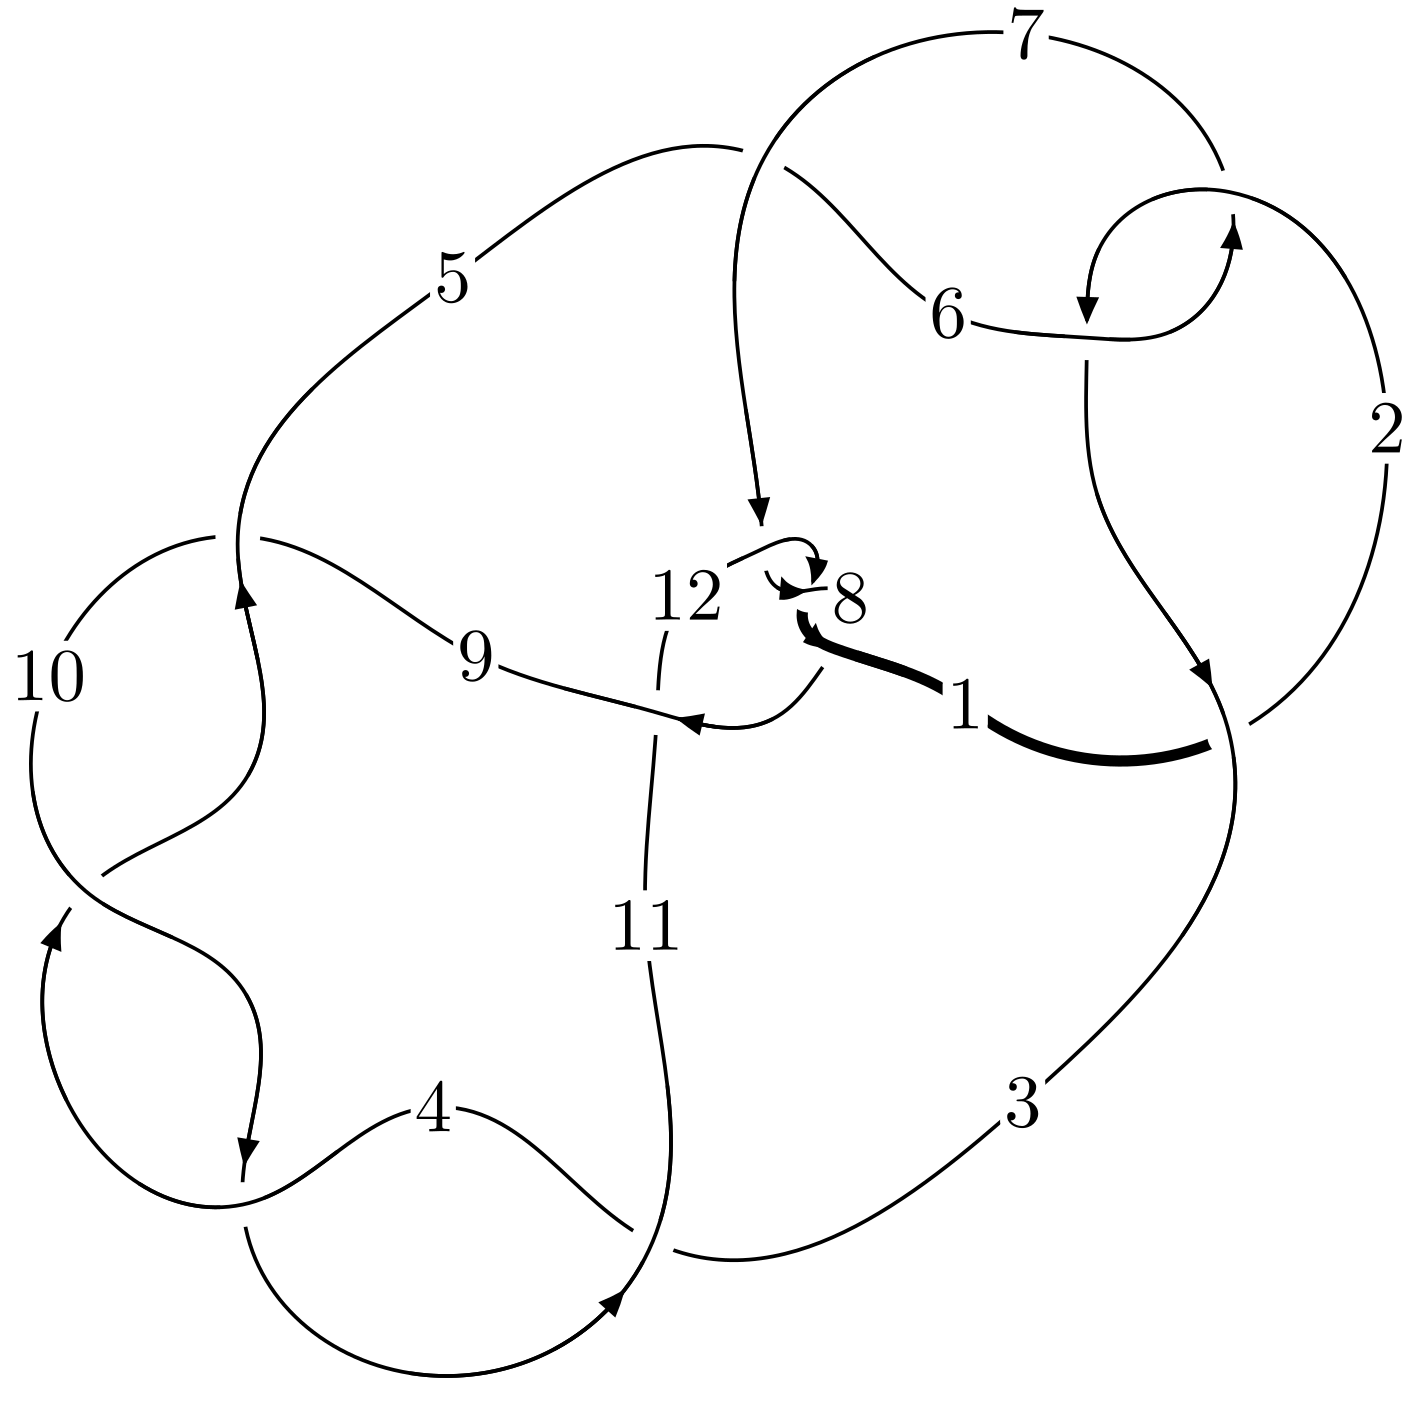
\includegraphics[width=112pt]{../../../GIT/diagram.site/Diagrams/png/1282_12a_0481.png}\\
\ \ \ A knot diagram\footnotemark}&
\allowdisplaybreaks
\textbf{Linearized knot diagam} \\
\cline{2-2}
 &
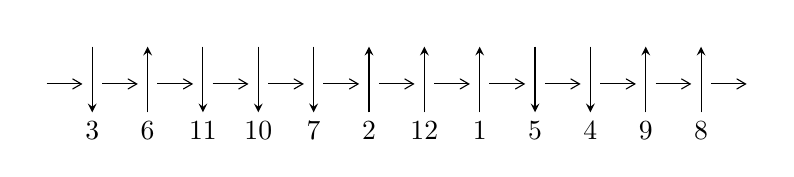
\begin{tikzpicture}[x=20pt, y=17pt]
	% nodes
	\node (C0) at (0, 0) {};
	\node (C1) at (1, 0) {};
	\node (C1U) at (1, +1) {};
	\node (C1D) at (1, -1) {3};

	\node (C2) at (2, 0) {};
	\node (C2U) at (2, +1) {};
	\node (C2D) at (2, -1) {6};

	\node (C3) at (3, 0) {};
	\node (C3U) at (3, +1) {};
	\node (C3D) at (3, -1) {11};

	\node (C4) at (4, 0) {};
	\node (C4U) at (4, +1) {};
	\node (C4D) at (4, -1) {10};

	\node (C5) at (5, 0) {};
	\node (C5U) at (5, +1) {};
	\node (C5D) at (5, -1) {7};

	\node (C6) at (6, 0) {};
	\node (C6U) at (6, +1) {};
	\node (C6D) at (6, -1) {2};

	\node (C7) at (7, 0) {};
	\node (C7U) at (7, +1) {};
	\node (C7D) at (7, -1) {12};

	\node (C8) at (8, 0) {};
	\node (C8U) at (8, +1) {};
	\node (C8D) at (8, -1) {1};

	\node (C9) at (9, 0) {};
	\node (C9U) at (9, +1) {};
	\node (C9D) at (9, -1) {5};

	\node (C10) at (10, 0) {};
	\node (C10U) at (10, +1) {};
	\node (C10D) at (10, -1) {4};

	\node (C11) at (11, 0) {};
	\node (C11U) at (11, +1) {};
	\node (C11D) at (11, -1) {9};

	\node (C12) at (12, 0) {};
	\node (C12U) at (12, +1) {};
	\node (C12D) at (12, -1) {8};
	\node (C13) at (13, 0) {};

	% arrows
	\draw[->,>={angle 60}]
	(C0) edge (C1) (C1) edge (C2) (C2) edge (C3) (C3) edge (C4) (C4) edge (C5) (C5) edge (C6) (C6) edge (C7) (C7) edge (C8) (C8) edge (C9) (C9) edge (C10) (C10) edge (C11) (C11) edge (C12) (C12) edge (C13) ;	\draw[->,>=stealth]
	(C1U) edge (C1D) (C2D) edge (C2U) (C3U) edge (C3D) (C4U) edge (C4D) (C5U) edge (C5D) (C6D) edge (C6U) (C7D) edge (C7U) (C8D) edge (C8U) (C9U) edge (C9D) (C10U) edge (C10D) (C11D) edge (C11U) (C12D) edge (C12U) ;
	\end{tikzpicture} \\
\hhline{~~} \\& 
\textbf{Solving Sequence} \\ \cline{2-2} 
 &
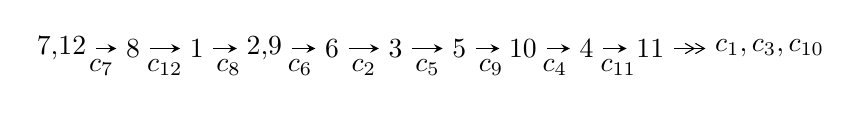
\begin{tikzpicture}[x=23pt, y=7pt]
	% node
	\node (A0) at (-1/8, 0) {7,12};
	\node (A1) at (1, 0) {8};
	\node (A2) at (2, 0) {1};
	\node (A3) at (49/16, 0) {2,9};
	\node (A4) at (33/8, 0) {6};
	\node (A5) at (41/8, 0) {3};
	\node (A6) at (49/8, 0) {5};
	\node (A7) at (57/8, 0) {10};
	\node (A8) at (65/8, 0) {4};
	\node (A9) at (73/8, 0) {11};
	\node (C1) at (1/2, -1) {$c_{7}$};
	\node (C2) at (3/2, -1) {$c_{12}$};
	\node (C3) at (5/2, -1) {$c_{8}$};
	\node (C4) at (29/8, -1) {$c_{6}$};
	\node (C5) at (37/8, -1) {$c_{2}$};
	\node (C6) at (45/8, -1) {$c_{5}$};
	\node (C7) at (53/8, -1) {$c_{9}$};
	\node (C8) at (61/8, -1) {$c_{4}$};
	\node (C9) at (69/8, -1) {$c_{11}$};
	\node (A10) at (11, 0) {$c_{1},c_{3},c_{10}$};

	% edge
	\draw[->,>=stealth]	
	(A0) edge (A1) (A1) edge (A2) (A2) edge (A3) (A3) edge (A4) (A4) edge (A5) (A5) edge (A6) (A6) edge (A7) (A7) edge (A8) (A8) edge (A9) ;
	\draw[->>,>={angle 60}]	
	(A9) edge (A10);
\end{tikzpicture} \\ 

\end{tabular} \\

\footnotetext{
The image of knot diagram is generated by the software ``\textbf{Draw programme}" developed by Andrew Bartholomew(\url{http://www.layer8.co.uk/maths/draw/index.htm\#Running-draw}), where we modified some parts for our purpose(\url{https://github.com/CATsTAILs/LinksPainter}).
}\phantom \\ \newline 
\centering \textbf{Ideals for irreducible components\footnotemark of $X_{\text{par}}$} 
 
\begin{align*}
I^u_{1}&=\langle 
8.33546\times10^{45} u^{64}-1.14445\times10^{46} u^{63}+\cdots+2.27514\times10^{46} b+7.73936\times10^{46},\\
\phantom{I^u_{1}}&\phantom{= \langle  }-6.97340\times10^{45} u^{64}+1.87570\times10^{46} u^{63}+\cdots+6.82541\times10^{45} a-1.64156\times10^{46},\;u^{65}-3 u^{64}+\cdots-8 u-3\rangle \\
I^u_{2}&=\langle 
a^2+2 b-2 a+1,\;a^4-4 a^3+4 a^2+3,\;u-1\rangle \\
I^u_{3}&=\langle 
b^2- b+1,\;a+1,\;u+1\rangle \\
\\
\end{align*}
\raggedright * 3 irreducible components of $\dim_{\mathbb{C}}=0$, with total 71 representations.\\
\footnotetext{All coefficients of polynomials are rational numbers. But the coefficients are sometimes approximated in decimal forms when there is not enough margin.}
\newpage
\renewcommand{\arraystretch}{1}
\centering \section*{I. $I^u_{1}= \langle 8.34\times10^{45} u^{64}-1.14\times10^{46} u^{63}+\cdots+2.28\times10^{46} b+7.74\times10^{46},\;-6.97\times10^{45} u^{64}+1.88\times10^{46} u^{63}+\cdots+6.83\times10^{45} a-1.64\times10^{46},\;u^{65}-3 u^{64}+\cdots-8 u-3 \rangle$}
\flushleft \textbf{(i) Arc colorings}\\
\begin{tabular}{m{7pt} m{180pt} m{7pt} m{180pt} }
\flushright $a_{7}=$&$\begin{pmatrix}1\\0\end{pmatrix}$ \\
\flushright $a_{12}=$&$\begin{pmatrix}0\\u\end{pmatrix}$ \\
\flushright $a_{8}=$&$\begin{pmatrix}1\\- u^2\end{pmatrix}$ \\
\flushright $a_{1}=$&$\begin{pmatrix}u\\- u^3+u\end{pmatrix}$ \\
\flushright $a_{2}=$&$\begin{pmatrix}1.02168 u^{64}-2.74811 u^{63}+\cdots-15.6860 u+2.40507\\-0.366372 u^{64}+0.503023 u^{63}+\cdots-12.2381 u-3.40171\end{pmatrix}$ \\
\flushright $a_{9}=$&$\begin{pmatrix}- u^2+1\\u^4-2 u^2\end{pmatrix}$ \\
\flushright $a_{6}=$&$\begin{pmatrix}1.66172 u^{64}-2.35528 u^{63}+\cdots+8.61379 u-3.26790\\-0.319726 u^{64}+0.744780 u^{63}+\cdots+1.79163 u-1.12739\end{pmatrix}$ \\
\flushright $a_{3}=$&$\begin{pmatrix}2.25408 u^{64}-3.92752 u^{63}+\cdots+15.8897 u+9.78314\\-1.38909 u^{64}+1.98660 u^{63}+\cdots-19.4141 u-3.51898\end{pmatrix}$ \\
\flushright $a_{5}=$&$\begin{pmatrix}1.34199 u^{64}-1.61050 u^{63}+\cdots+10.4054 u-4.39529\\-0.319726 u^{64}+0.744780 u^{63}+\cdots+1.79163 u-1.12739\end{pmatrix}$ \\
\flushright $a_{10}=$&$\begin{pmatrix}1.60989 u^{64}-4.21548 u^{63}+\cdots-32.4505 u-3.49651\\-0.276179 u^{64}+0.246100 u^{63}+\cdots-7.07338 u-3.16209\end{pmatrix}$ \\
\flushright $a_{4}=$&$\begin{pmatrix}1.03866 u^{64}-1.95917 u^{63}+\cdots+7.94157 u+7.99324\\-0.995853 u^{64}+1.35764 u^{63}+\cdots-16.0888 u-2.99309\end{pmatrix}$ \\
\flushright $a_{11}=$&$\begin{pmatrix}- u^5+2 u^3- u\\u^7-3 u^5+2 u^3+u\end{pmatrix}$\\&\end{tabular}
\flushleft \textbf{(ii) Obstruction class $= -1$}\\~\\
\flushleft \textbf{(iii) Cusp Shapes $= 0.575409 u^{64}-1.03751 u^{63}+\cdots-12.2400 u+0.321049$}\\~\\
\newpage\renewcommand{\arraystretch}{1}
\flushleft \textbf{(iv) u-Polynomials at the component}\newline \\
\begin{tabular}{m{50pt}|m{274pt}}
Crossings & \hspace{64pt}u-Polynomials at each crossing \\
\hline $$\begin{aligned}c_{1},c_{5}\end{aligned}$$&$\begin{aligned}
&u^{65}+22 u^{64}+\cdots-29 u-9
\end{aligned}$\\
\hline $$\begin{aligned}c_{2},c_{6}\end{aligned}$$&$\begin{aligned}
&u^{65}-2 u^{64}+\cdots- u+3
\end{aligned}$\\
\hline $$\begin{aligned}c_{3},c_{4},c_{9}\\c_{10}\end{aligned}$$&$\begin{aligned}
&u^{65}+u^{64}+\cdots-16 u-4
\end{aligned}$\\
\hline $$\begin{aligned}c_{7},c_{8},c_{12}\end{aligned}$$&$\begin{aligned}
&u^{65}-3 u^{64}+\cdots-8 u-3
\end{aligned}$\\
\hline $$\begin{aligned}c_{11}\end{aligned}$$&$\begin{aligned}
&u^{65}+15 u^{64}+\cdots+9984 u+2304
\end{aligned}$\\
\hline
\end{tabular}\\~\\
\newpage\renewcommand{\arraystretch}{1}
\flushleft \textbf{(v) Riley Polynomials at the component}\newline \\
\begin{tabular}{m{50pt}|m{274pt}}
Crossings & \hspace{64pt}Riley Polynomials at each crossing \\
\hline $$\begin{aligned}c_{1},c_{5}\end{aligned}$$&$\begin{aligned}
&y^{65}+46 y^{64}+\cdots-2741 y-81
\end{aligned}$\\
\hline $$\begin{aligned}c_{2},c_{6}\end{aligned}$$&$\begin{aligned}
&y^{65}+22 y^{64}+\cdots-29 y-9
\end{aligned}$\\
\hline $$\begin{aligned}c_{3},c_{4},c_{9}\\c_{10}\end{aligned}$$&$\begin{aligned}
&y^{65}+75 y^{64}+\cdots-192 y-16
\end{aligned}$\\
\hline $$\begin{aligned}c_{7},c_{8},c_{12}\end{aligned}$$&$\begin{aligned}
&y^{65}-59 y^{64}+\cdots-248 y-9
\end{aligned}$\\
\hline $$\begin{aligned}c_{11}\end{aligned}$$&$\begin{aligned}
&y^{65}- y^{64}+\cdots-97026048 y-5308416
\end{aligned}$\\
\hline
\end{tabular}\\~\\
\newpage\flushleft \textbf{(vi) Complex Volumes and Cusp Shapes}
$$\begin{array}{c|c|c}  
\text{Solutions to }I^u_{1}& \I (\text{vol} + \sqrt{-1}CS) & \text{Cusp shape}\\
 \hline 
\begin{aligned}
u &= \phantom{-}0.888082 + 0.410833 I \\
a &= \phantom{-}0.646410 - 0.203115 I \\
b &= -0.654237 + 0.917487 I\end{aligned}
 & \phantom{-}2.60919 - 2.94570 I & \phantom{-}5.59381 + 4.95414 I \\ \hline\begin{aligned}
u &= \phantom{-}0.888082 - 0.410833 I \\
a &= \phantom{-}0.646410 + 0.203115 I \\
b &= -0.654237 - 0.917487 I\end{aligned}
 & \phantom{-}2.60919 + 2.94570 I & \phantom{-}5.59381 - 4.95414 I \\ \hline\begin{aligned}
u &= -0.303651 + 0.902592 I \\
a &= -1.11503 - 1.04244 I \\
b &= \phantom{-}0.723865 - 1.009450 I\end{aligned}
 & \phantom{-}8.20289 - 9.66985 I & \phantom{-}4.28819 + 7.03671 I \\ \hline\begin{aligned}
u &= -0.303651 - 0.902592 I \\
a &= -1.11503 + 1.04244 I \\
b &= \phantom{-}0.723865 + 1.009450 I\end{aligned}
 & \phantom{-}8.20289 + 9.66985 I & \phantom{-}4.28819 - 7.03671 I \\ \hline\begin{aligned}
u &= -0.357028 + 0.864794 I \\
a &= -0.120170 - 0.184351 I \\
b &= \phantom{-}0.810435 + 0.695902 I\end{aligned}
 & \phantom{-}9.15604 - 3.90043 I & \phantom{-}6.04015 + 2.26901 I \\ \hline\begin{aligned}
u &= -0.357028 - 0.864794 I \\
a &= -0.120170 + 0.184351 I \\
b &= \phantom{-}0.810435 - 0.695902 I\end{aligned}
 & \phantom{-}9.15604 + 3.90043 I & \phantom{-}6.04015 - 2.26901 I \\ \hline\begin{aligned}
u &= -0.871939 + 0.644664 I \\
a &= -1.166130 - 0.395613 I \\
b &= \phantom{-}0.775582 - 0.780086 I\end{aligned}
 & \phantom{-}10.69910 - 1.33054 I & \phantom{-0.000000 } 0 \\ \hline\begin{aligned}
u &= -0.871939 - 0.644664 I \\
a &= -1.166130 + 0.395613 I \\
b &= \phantom{-}0.775582 + 0.780086 I\end{aligned}
 & \phantom{-}10.69910 + 1.33054 I & \phantom{-0.000000 } 0 \\ \hline\begin{aligned}
u &= -1.071940 + 0.271690 I \\
a &= -1.51716 - 0.45745 I \\
b &= -0.059410 - 0.833219 I\end{aligned}
 & \phantom{-}5.29432 + 0.38771 I & \phantom{-0.000000 } 0 \\ \hline\begin{aligned}
u &= -1.071940 - 0.271690 I \\
a &= -1.51716 + 0.45745 I \\
b &= -0.059410 + 0.833219 I\end{aligned}
 & \phantom{-}5.29432 - 0.38771 I & \phantom{-0.000000 } 0\\
 \hline 
 \end{array}$$\newpage$$\begin{array}{c|c|c}  
\text{Solutions to }I^u_{1}& \I (\text{vol} + \sqrt{-1}CS) & \text{Cusp shape}\\
 \hline 
\begin{aligned}
u &= -0.956232 + 0.622330 I \\
a &= -0.508319 - 0.122319 I \\
b &= \phantom{-}0.730631 + 0.950916 I\end{aligned}
 & \phantom{-}10.17330 + 4.36468 I & \phantom{-0.000000 } 0 \\ \hline\begin{aligned}
u &= -0.956232 - 0.622330 I \\
a &= -0.508319 + 0.122319 I \\
b &= \phantom{-}0.730631 - 0.950916 I\end{aligned}
 & \phantom{-}10.17330 - 4.36468 I & \phantom{-0.000000 } 0 \\ \hline\begin{aligned}
u &= \phantom{-}0.746987 + 0.405773 I \\
a &= \phantom{-}1.373230 - 0.240037 I \\
b &= -0.663828 - 0.797440 I\end{aligned}
 & \phantom{-}2.98112 + 2.17079 I & \phantom{-}7.43307 - 2.82107 I \\ \hline\begin{aligned}
u &= \phantom{-}0.746987 - 0.405773 I \\
a &= \phantom{-}1.373230 + 0.240037 I \\
b &= -0.663828 + 0.797440 I\end{aligned}
 & \phantom{-}2.98112 - 2.17079 I & \phantom{-}7.43307 + 2.82107 I \\ \hline\begin{aligned}
u &= \phantom{-}0.262619 + 0.779561 I \\
a &= \phantom{-}1.28732 - 1.13527 I \\
b &= -0.685423 - 0.989058 I\end{aligned}
 & \phantom{-}0.66485 + 7.27591 I & \phantom{-}1.08861 - 8.89845 I \\ \hline\begin{aligned}
u &= \phantom{-}0.262619 - 0.779561 I \\
a &= \phantom{-}1.28732 + 1.13527 I \\
b &= -0.685423 + 0.989058 I\end{aligned}
 & \phantom{-}0.66485 - 7.27591 I & \phantom{-}1.08861 + 8.89845 I \\ \hline\begin{aligned}
u &= \phantom{-}1.20544\phantom{ +0.000000I} \\
a &= \phantom{-}1.04693\phantom{ +0.000000I} \\
b &= -0.442541\phantom{ +0.000000I}\end{aligned}
 & \phantom{-}2.51098\phantom{ +0.000000I} & \phantom{-0.000000 } 0 \\ \hline\begin{aligned}
u &= -1.210530 + 0.121438 I \\
a &= -0.804093 + 0.106541 I \\
b &= \phantom{-}0.485668 + 1.012200 I\end{aligned}
 & \phantom{-}2.34586 + 1.24708 I & \phantom{-0.000000 } 0 \\ \hline\begin{aligned}
u &= -1.210530 - 0.121438 I \\
a &= -0.804093 - 0.106541 I \\
b &= \phantom{-}0.485668 - 1.012200 I\end{aligned}
 & \phantom{-}2.34586 - 1.24708 I & \phantom{-0.000000 } 0 \\ \hline\begin{aligned}
u &= \phantom{-}1.189940 + 0.262812 I \\
a &= \phantom{-}1.112030 - 0.471723 I \\
b &= -0.102185 - 0.962937 I\end{aligned}
 & -0.41777 + 1.70342 I & \phantom{-0.000000 } 0\\
 \hline 
 \end{array}$$\newpage$$\begin{array}{c|c|c}  
\text{Solutions to }I^u_{1}& \I (\text{vol} + \sqrt{-1}CS) & \text{Cusp shape}\\
 \hline 
\begin{aligned}
u &= \phantom{-}1.189940 - 0.262812 I \\
a &= \phantom{-}1.112030 + 0.471723 I \\
b &= -0.102185 + 0.962937 I\end{aligned}
 & -0.41777 - 1.70342 I & \phantom{-0.000000 } 0 \\ \hline\begin{aligned}
u &= \phantom{-}0.300846 + 0.705195 I \\
a &= \phantom{-}0.041328 - 0.304729 I \\
b &= -0.729277 + 0.685600 I\end{aligned}
 & \phantom{-}1.57098 + 1.85327 I & \phantom{-}3.17798 - 4.14987 I \\ \hline\begin{aligned}
u &= \phantom{-}0.300846 - 0.705195 I \\
a &= \phantom{-}0.041328 + 0.304729 I \\
b &= -0.729277 - 0.685600 I\end{aligned}
 & \phantom{-}1.57098 - 1.85327 I & \phantom{-}3.17798 + 4.14987 I \\ \hline\begin{aligned}
u &= -0.196519 + 0.709917 I \\
a &= -0.04566 + 1.82055 I \\
b &= -0.140059 + 1.043640 I\end{aligned}
 & \phantom{-}2.74271 - 4.03109 I & -1.56032 + 4.30145 I \\ \hline\begin{aligned}
u &= -0.196519 - 0.709917 I \\
a &= -0.04566 - 1.82055 I \\
b &= -0.140059 - 1.043640 I\end{aligned}
 & \phantom{-}2.74271 + 4.03109 I & -1.56032 - 4.30145 I \\ \hline\begin{aligned}
u &= \phantom{-}0.062464 + 0.696936 I \\
a &= \phantom{-}0.03481 + 1.70684 I \\
b &= \phantom{-}0.048122 + 1.014310 I\end{aligned}
 & -3.83534 + 1.80189 I & -6.00427 - 4.43623 I \\ \hline\begin{aligned}
u &= \phantom{-}0.062464 - 0.696936 I \\
a &= \phantom{-}0.03481 - 1.70684 I \\
b &= \phantom{-}0.048122 - 1.014310 I\end{aligned}
 & -3.83534 - 1.80189 I & -6.00427 + 4.43623 I \\ \hline\begin{aligned}
u &= -0.414473 + 0.549756 I \\
a &= -0.258906 + 0.215659 I \\
b &= -0.577074 + 0.179072 I\end{aligned}
 & \phantom{-}6.60099 - 1.84186 I & \phantom{-}5.73903 + 3.43368 I \\ \hline\begin{aligned}
u &= -0.414473 - 0.549756 I \\
a &= -0.258906 - 0.215659 I \\
b &= -0.577074 - 0.179072 I\end{aligned}
 & \phantom{-}6.60099 + 1.84186 I & \phantom{-}5.73903 - 3.43368 I \\ \hline\begin{aligned}
u &= -1.297190 + 0.268858 I \\
a &= -0.933747 - 0.495340 I \\
b &= \phantom{-}0.150814 - 1.077000 I\end{aligned}
 & \phantom{-}0.40210 - 5.28798 I & \phantom{-0.000000 } 0\\
 \hline 
 \end{array}$$\newpage$$\begin{array}{c|c|c}  
\text{Solutions to }I^u_{1}& \I (\text{vol} + \sqrt{-1}CS) & \text{Cusp shape}\\
 \hline 
\begin{aligned}
u &= -1.297190 - 0.268858 I \\
a &= -0.933747 + 0.495340 I \\
b &= \phantom{-}0.150814 + 1.077000 I\end{aligned}
 & \phantom{-}0.40210 + 5.28798 I & \phantom{-0.000000 } 0 \\ \hline\begin{aligned}
u &= -1.317890 + 0.155610 I \\
a &= -1.011440 - 0.057697 I \\
b &= \phantom{-}0.665716 - 0.212271 I\end{aligned}
 & \phantom{-}4.57403 - 2.83927 I & \phantom{-0.000000 } 0 \\ \hline\begin{aligned}
u &= -1.317890 - 0.155610 I \\
a &= -1.011440 + 0.057697 I \\
b &= \phantom{-}0.665716 + 0.212271 I\end{aligned}
 & \phantom{-}4.57403 + 2.83927 I & \phantom{-0.000000 } 0 \\ \hline\begin{aligned}
u &= -0.207623 + 0.592264 I \\
a &= -1.69337 - 1.29542 I \\
b &= \phantom{-}0.633445 - 0.958857 I\end{aligned}
 & -0.43277 - 3.63822 I & -2.67168 + 3.01987 I \\ \hline\begin{aligned}
u &= -0.207623 - 0.592264 I \\
a &= -1.69337 + 1.29542 I \\
b &= \phantom{-}0.633445 + 0.958857 I\end{aligned}
 & -0.43277 + 3.63822 I & -2.67168 - 3.01987 I \\ \hline\begin{aligned}
u &= \phantom{-}1.373270 + 0.150068 I \\
a &= \phantom{-}0.714513 + 0.181428 I \\
b &= -0.483932 + 1.111580 I\end{aligned}
 & \phantom{-}9.70090 - 0.05073 I & \phantom{-0.000000 } 0 \\ \hline\begin{aligned}
u &= \phantom{-}1.373270 - 0.150068 I \\
a &= \phantom{-}0.714513 - 0.181428 I \\
b &= -0.483932 - 1.111580 I\end{aligned}
 & \phantom{-}9.70090 + 0.05073 I & \phantom{-0.000000 } 0 \\ \hline\begin{aligned}
u &= -1.384540 + 0.118480 I \\
a &= \phantom{-}2.46352 - 0.66760 I \\
b &= -0.730700 + 0.918700 I\end{aligned}
 & \phantom{-}9.31806 - 3.11523 I & \phantom{-0.000000 } 0 \\ \hline\begin{aligned}
u &= -1.384540 - 0.118480 I \\
a &= \phantom{-}2.46352 + 0.66760 I \\
b &= -0.730700 - 0.918700 I\end{aligned}
 & \phantom{-}9.31806 + 3.11523 I & \phantom{-0.000000 } 0 \\ \hline\begin{aligned}
u &= \phantom{-}1.380960 + 0.184417 I \\
a &= -1.09435 + 1.47451 I \\
b &= \phantom{-}0.778406 - 0.728805 I\end{aligned}
 & \phantom{-}5.42221 + 1.04361 I & \phantom{-0.000000 } 0\\
 \hline 
 \end{array}$$\newpage$$\begin{array}{c|c|c}  
\text{Solutions to }I^u_{1}& \I (\text{vol} + \sqrt{-1}CS) & \text{Cusp shape}\\
 \hline 
\begin{aligned}
u &= \phantom{-}1.380960 - 0.184417 I \\
a &= -1.09435 - 1.47451 I \\
b &= \phantom{-}0.778406 + 0.728805 I\end{aligned}
 & \phantom{-}5.42221 - 1.04361 I & \phantom{-0.000000 } 0 \\ \hline\begin{aligned}
u &= \phantom{-}1.383180 + 0.238836 I \\
a &= -2.49505 - 0.01259 I \\
b &= \phantom{-}0.717910 + 0.982922 I\end{aligned}
 & \phantom{-}4.64807 + 6.70673 I & \phantom{-0.000000 } 0 \\ \hline\begin{aligned}
u &= \phantom{-}1.383180 - 0.238836 I \\
a &= -2.49505 + 0.01259 I \\
b &= \phantom{-}0.717910 - 0.982922 I\end{aligned}
 & \phantom{-}4.64807 - 6.70673 I & \phantom{-0.000000 } 0 \\ \hline\begin{aligned}
u &= -1.405930 + 0.052718 I \\
a &= \phantom{-}1.73085 + 1.30451 I \\
b &= -0.766620 - 0.820153 I\end{aligned}
 & \phantom{-}9.62594 + 2.55262 I & \phantom{-0.000000 } 0 \\ \hline\begin{aligned}
u &= -1.405930 - 0.052718 I \\
a &= \phantom{-}1.73085 - 1.30451 I \\
b &= -0.766620 + 0.820153 I\end{aligned}
 & \phantom{-}9.62594 - 2.55262 I & \phantom{-0.000000 } 0 \\ \hline\begin{aligned}
u &= \phantom{-}1.384210 + 0.280090 I \\
a &= \phantom{-}0.831833 - 0.504549 I \\
b &= -0.172242 - 1.152380 I\end{aligned}
 & \phantom{-}7.78079 + 7.61615 I & \phantom{-0.000000 } 0 \\ \hline\begin{aligned}
u &= \phantom{-}1.384210 - 0.280090 I \\
a &= \phantom{-}0.831833 + 0.504549 I \\
b &= -0.172242 + 1.152380 I\end{aligned}
 & \phantom{-}7.78079 - 7.61615 I & \phantom{-0.000000 } 0 \\ \hline\begin{aligned}
u &= -1.41598 + 0.27122 I \\
a &= \phantom{-}0.83745 + 1.23150 I \\
b &= -0.827312 - 0.681734 I\end{aligned}
 & \phantom{-}7.04530 - 5.39041 I & \phantom{-0.000000 } 0 \\ \hline\begin{aligned}
u &= -1.41598 - 0.27122 I \\
a &= \phantom{-}0.83745 - 1.23150 I \\
b &= -0.827312 + 0.681734 I\end{aligned}
 & \phantom{-}7.04530 + 5.39041 I & \phantom{-0.000000 } 0 \\ \hline\begin{aligned}
u &= \phantom{-}1.43155 + 0.20492 I \\
a &= \phantom{-}0.966638 - 0.073545 I \\
b &= -0.809524 - 0.220320 I\end{aligned}
 & \phantom{-}12.46300 + 4.59312 I & \phantom{-0.000000 } 0\\
 \hline 
 \end{array}$$\newpage$$\begin{array}{c|c|c}  
\text{Solutions to }I^u_{1}& \I (\text{vol} + \sqrt{-1}CS) & \text{Cusp shape}\\
 \hline 
\begin{aligned}
u &= \phantom{-}1.43155 - 0.20492 I \\
a &= \phantom{-}0.966638 + 0.073545 I \\
b &= -0.809524 + 0.220320 I\end{aligned}
 & \phantom{-}12.46300 - 4.59312 I & \phantom{-0.000000 } 0 \\ \hline\begin{aligned}
u &= -1.41407 + 0.30946 I \\
a &= \phantom{-}2.26793 + 0.23939 I \\
b &= -0.726429 + 1.021480 I\end{aligned}
 & \phantom{-}6.01152 - 11.21260 I & \phantom{-0.000000 } 0 \\ \hline\begin{aligned}
u &= -1.41407 - 0.30946 I \\
a &= \phantom{-}2.26793 - 0.23939 I \\
b &= -0.726429 - 1.021480 I\end{aligned}
 & \phantom{-}6.01152 + 11.21260 I & \phantom{-0.000000 } 0 \\ \hline\begin{aligned}
u &= \phantom{-}1.45455 + 0.36028 I \\
a &= -2.06306 + 0.33688 I \\
b &= \phantom{-}0.740697 + 1.050510 I\end{aligned}
 & \phantom{-}13.8214 + 14.2192 I & \phantom{-0.000000 } 0 \\ \hline\begin{aligned}
u &= \phantom{-}1.45455 - 0.36028 I \\
a &= -2.06306 - 0.33688 I \\
b &= \phantom{-}0.740697 - 1.050510 I\end{aligned}
 & \phantom{-}13.8214 - 14.2192 I & \phantom{-0.000000 } 0 \\ \hline\begin{aligned}
u &= \phantom{-}1.46756 + 0.32998 I \\
a &= -0.765398 + 1.035260 I \\
b &= \phantom{-}0.879332 - 0.662994 I\end{aligned}
 & \phantom{-}15.0130 + 8.2071 I & \phantom{-0.000000 } 0 \\ \hline\begin{aligned}
u &= \phantom{-}1.46756 - 0.32998 I \\
a &= -0.765398 - 1.035260 I \\
b &= \phantom{-}0.879332 + 0.662994 I\end{aligned}
 & \phantom{-}15.0130 - 8.2071 I & \phantom{-0.000000 } 0 \\ \hline\begin{aligned}
u &= -0.237234 + 0.386656 I \\
a &= \phantom{-}0.214919 - 0.937698 I \\
b &= \phantom{-}0.587428 + 0.735506 I\end{aligned}
 & \phantom{-}0.293265 + 1.243780 I & -2.51844 - 2.93595 I \\ \hline\begin{aligned}
u &= -0.237234 - 0.386656 I \\
a &= \phantom{-}0.214919 + 0.937698 I \\
b &= \phantom{-}0.587428 - 0.735506 I\end{aligned}
 & \phantom{-}0.293265 - 1.243780 I & -2.51844 + 2.93595 I \\ \hline\begin{aligned}
u &= \phantom{-}1.56257 + 0.02370 I \\
a &= -1.62357 - 0.63557 I \\
b &= \phantom{-}0.843446 + 0.892821 I\end{aligned}
 & \phantom{-}19.3856 + 3.1221 I & \phantom{-0.000000 } 0\\
 \hline 
 \end{array}$$\newpage$$\begin{array}{c|c|c}  
\text{Solutions to }I^u_{1}& \I (\text{vol} + \sqrt{-1}CS) & \text{Cusp shape}\\
 \hline 
\begin{aligned}
u &= \phantom{-}1.56257 - 0.02370 I \\
a &= -1.62357 + 0.63557 I \\
b &= \phantom{-}0.843446 - 0.892821 I\end{aligned}
 & \phantom{-}19.3856 - 3.1221 I & \phantom{-0.000000 } 0 \\ \hline\begin{aligned}
u &= \phantom{-}0.172559 + 0.341650 I \\
a &= \phantom{-}0.289287 + 0.247747 I \\
b &= \phantom{-}0.296575 + 0.310433 I\end{aligned}
 & \phantom{-}0.059571 + 0.856042 I & \phantom{-}1.59029 - 7.87693 I \\ \hline\begin{aligned}
u &= \phantom{-}0.172559 - 0.341650 I \\
a &= \phantom{-}0.289287 - 0.247747 I \\
b &= \phantom{-}0.296575 - 0.310433 I\end{aligned}
 & \phantom{-}0.059571 - 0.856042 I & \phantom{-}1.59029 + 7.87693 I \\ \hline\begin{aligned}
u &= -0.101292 + 0.291578 I \\
a &= \phantom{-}2.21326 - 3.83264 I \\
b &= -0.518548 - 0.944155 I\end{aligned}
 & \phantom{-}4.81440 + 1.86541 I & -0.02684 - 2.78315 I \\ \hline\begin{aligned}
u &= -0.101292 - 0.291578 I \\
a &= \phantom{-}2.21326 + 3.83264 I \\
b &= -0.518548 + 0.944155 I\end{aligned}
 & \phantom{-}4.81440 - 1.86541 I & -0.02684 + 2.78315 I\\
 \hline 
 \end{array}$$\newpage\newpage\renewcommand{\arraystretch}{1}
\centering \section*{II. $I^u_{2}= \langle a^2+2 b-2 a+1,\;a^4-4 a^3+4 a^2+3,\;u-1 \rangle$}
\flushleft \textbf{(i) Arc colorings}\\
\begin{tabular}{m{7pt} m{180pt} m{7pt} m{180pt} }
\flushright $a_{7}=$&$\begin{pmatrix}1\\0\end{pmatrix}$ \\
\flushright $a_{12}=$&$\begin{pmatrix}0\\1\end{pmatrix}$ \\
\flushright $a_{8}=$&$\begin{pmatrix}1\\-1\end{pmatrix}$ \\
\flushright $a_{1}=$&$\begin{pmatrix}1\\0\end{pmatrix}$ \\
\flushright $a_{2}=$&$\begin{pmatrix}a\\-\frac{1}{2} a^2+a-\frac{1}{2}\end{pmatrix}$ \\
\flushright $a_{9}=$&$\begin{pmatrix}0\\-1\end{pmatrix}$ \\
\flushright $a_{6}=$&$\begin{pmatrix}-\frac{1}{2} a^3+a^2-\frac{1}{2} a+1\\\frac{1}{2} a^2- a-\frac{1}{2}\end{pmatrix}$ \\
\flushright $a_{3}=$&$\begin{pmatrix}\frac{1}{2} a^3-\frac{3}{2} a^2+\frac{3}{2} a-\frac{1}{2}\\-\frac{1}{2} a^2+a+\frac{1}{2}\end{pmatrix}$ \\
\flushright $a_{5}=$&$\begin{pmatrix}-\frac{1}{2} a^3+\frac{3}{2} a^2-\frac{3}{2} a+\frac{1}{2}\\\frac{1}{2} a^2- a-\frac{1}{2}\end{pmatrix}$ \\
\flushright $a_{10}=$&$\begin{pmatrix}-2\\a-2\end{pmatrix}$ \\
\flushright $a_{4}=$&$\begin{pmatrix}\frac{1}{2} a^3-\frac{3}{2} a^2+\frac{3}{2} a-\frac{1}{2}\\\frac{1}{2} a^3-2 a^2+\frac{5}{2} a\end{pmatrix}$ \\
\flushright $a_{11}=$&$\begin{pmatrix}0\\1\end{pmatrix}$\\&\end{tabular}
\flushleft \textbf{(ii) Obstruction class $= 1$}\\~\\
\flushleft \textbf{(iii) Cusp Shapes $= -2 a^2+4 a+6$}\\~\\
\newpage\renewcommand{\arraystretch}{1}
\flushleft \textbf{(iv) u-Polynomials at the component}\newline \\
\begin{tabular}{m{50pt}|m{274pt}}
Crossings & \hspace{64pt}u-Polynomials at each crossing \\
\hline $$\begin{aligned}c_{1},c_{2},c_{5}\end{aligned}$$&$\begin{aligned}
&(u^2- u+1)^2
\end{aligned}$\\
\hline $$\begin{aligned}c_{3},c_{4},c_{9}\\c_{10}\end{aligned}$$&$\begin{aligned}
&(u^2+2)^2
\end{aligned}$\\
\hline $$\begin{aligned}c_{6}\end{aligned}$$&$\begin{aligned}
&(u^2+u+1)^2
\end{aligned}$\\
\hline $$\begin{aligned}c_{7},c_{8}\end{aligned}$$&$\begin{aligned}
&(u-1)^4
\end{aligned}$\\
\hline $$\begin{aligned}c_{11}\end{aligned}$$&$\begin{aligned}
&u^4
\end{aligned}$\\
\hline $$\begin{aligned}c_{12}\end{aligned}$$&$\begin{aligned}
&(u+1)^4
\end{aligned}$\\
\hline
\end{tabular}\\~\\
\newpage\renewcommand{\arraystretch}{1}
\flushleft \textbf{(v) Riley Polynomials at the component}\newline \\
\begin{tabular}{m{50pt}|m{274pt}}
Crossings & \hspace{64pt}Riley Polynomials at each crossing \\
\hline $$\begin{aligned}c_{1},c_{2},c_{5}\\c_{6}\end{aligned}$$&$\begin{aligned}
&(y^2+y+1)^2
\end{aligned}$\\
\hline $$\begin{aligned}c_{3},c_{4},c_{9}\\c_{10}\end{aligned}$$&$\begin{aligned}
&(y+2)^4
\end{aligned}$\\
\hline $$\begin{aligned}c_{7},c_{8},c_{12}\end{aligned}$$&$\begin{aligned}
&(y-1)^4
\end{aligned}$\\
\hline $$\begin{aligned}c_{11}\end{aligned}$$&$\begin{aligned}
&y^4
\end{aligned}$\\
\hline
\end{tabular}\\~\\
\newpage\flushleft \textbf{(vi) Complex Volumes and Cusp Shapes}
$$\begin{array}{c|c|c}  
\text{Solutions to }I^u_{2}& \I (\text{vol} + \sqrt{-1}CS) & \text{Cusp shape}\\
 \hline 
\begin{aligned}
u &= \phantom{-}1.00000\phantom{ +0.000000I} \\
a &= -0.224745 + 0.707107 I \\
b &= -0.500000 + 0.866025 I\end{aligned}
 & \phantom{-}6.57974 - 2.02988 I & \phantom{-}6.00000 + 3.46410 I \\ \hline\begin{aligned}
u &= \phantom{-}1.00000\phantom{ +0.000000I} \\
a &= -0.224745 - 0.707107 I \\
b &= -0.500000 - 0.866025 I\end{aligned}
 & \phantom{-}6.57974 + 2.02988 I & \phantom{-}6.00000 - 3.46410 I \\ \hline\begin{aligned}
u &= \phantom{-}1.00000\phantom{ +0.000000I} \\
a &= \phantom{-}2.22474 + 0.70711 I \\
b &= -0.500000 - 0.866025 I\end{aligned}
 & \phantom{-}6.57974 + 2.02988 I & \phantom{-}6.00000 - 3.46410 I \\ \hline\begin{aligned}
u &= \phantom{-}1.00000\phantom{ +0.000000I} \\
a &= \phantom{-}2.22474 - 0.70711 I \\
b &= -0.500000 + 0.866025 I\end{aligned}
 & \phantom{-}6.57974 - 2.02988 I & \phantom{-}6.00000 + 3.46410 I\\
 \hline 
 \end{array}$$\newpage\newpage\renewcommand{\arraystretch}{1}
\centering \section*{III. $I^u_{3}= \langle b^2- b+1,\;a+1,\;u+1 \rangle$}
\flushleft \textbf{(i) Arc colorings}\\
\begin{tabular}{m{7pt} m{180pt} m{7pt} m{180pt} }
\flushright $a_{7}=$&$\begin{pmatrix}1\\0\end{pmatrix}$ \\
\flushright $a_{12}=$&$\begin{pmatrix}0\\-1\end{pmatrix}$ \\
\flushright $a_{8}=$&$\begin{pmatrix}1\\-1\end{pmatrix}$ \\
\flushright $a_{1}=$&$\begin{pmatrix}-1\\0\end{pmatrix}$ \\
\flushright $a_{2}=$&$\begin{pmatrix}-1\\b\end{pmatrix}$ \\
\flushright $a_{9}=$&$\begin{pmatrix}0\\-1\end{pmatrix}$ \\
\flushright $a_{6}=$&$\begin{pmatrix}- b+1\\b-1\end{pmatrix}$ \\
\flushright $a_{3}=$&$\begin{pmatrix}0\\b-1\end{pmatrix}$ \\
\flushright $a_{5}=$&$\begin{pmatrix}0\\b-1\end{pmatrix}$ \\
\flushright $a_{10}=$&$\begin{pmatrix}0\\-1\end{pmatrix}$ \\
\flushright $a_{4}=$&$\begin{pmatrix}0\\b-1\end{pmatrix}$ \\
\flushright $a_{11}=$&$\begin{pmatrix}0\\-1\end{pmatrix}$\\&\end{tabular}
\flushleft \textbf{(ii) Obstruction class $= 1$}\\~\\
\flushleft \textbf{(iii) Cusp Shapes $= -4 b+2$}\\~\\
\newpage\renewcommand{\arraystretch}{1}
\flushleft \textbf{(iv) u-Polynomials at the component}\newline \\
\begin{tabular}{m{50pt}|m{274pt}}
Crossings & \hspace{64pt}u-Polynomials at each crossing \\
\hline $$\begin{aligned}c_{1},c_{5},c_{6}\end{aligned}$$&$\begin{aligned}
&u^2- u+1
\end{aligned}$\\
\hline $$\begin{aligned}c_{2}\end{aligned}$$&$\begin{aligned}
&u^2+u+1
\end{aligned}$\\
\hline $$\begin{aligned}c_{3},c_{4},c_{9}\\c_{10},c_{11}\end{aligned}$$&$\begin{aligned}
&u^2
\end{aligned}$\\
\hline $$\begin{aligned}c_{7},c_{8}\end{aligned}$$&$\begin{aligned}
&(u+1)^2
\end{aligned}$\\
\hline $$\begin{aligned}c_{12}\end{aligned}$$&$\begin{aligned}
&(u-1)^2
\end{aligned}$\\
\hline
\end{tabular}\\~\\
\newpage\renewcommand{\arraystretch}{1}
\flushleft \textbf{(v) Riley Polynomials at the component}\newline \\
\begin{tabular}{m{50pt}|m{274pt}}
Crossings & \hspace{64pt}Riley Polynomials at each crossing \\
\hline $$\begin{aligned}c_{1},c_{2},c_{5}\\c_{6}\end{aligned}$$&$\begin{aligned}
&y^2+y+1
\end{aligned}$\\
\hline $$\begin{aligned}c_{3},c_{4},c_{9}\\c_{10},c_{11}\end{aligned}$$&$\begin{aligned}
&y^2
\end{aligned}$\\
\hline $$\begin{aligned}c_{7},c_{8},c_{12}\end{aligned}$$&$\begin{aligned}
&(y-1)^2
\end{aligned}$\\
\hline
\end{tabular}\\~\\
\newpage\flushleft \textbf{(vi) Complex Volumes and Cusp Shapes}
$$\begin{array}{c|c|c}  
\text{Solutions to }I^u_{3}& \I (\text{vol} + \sqrt{-1}CS) & \text{Cusp shape}\\
 \hline 
\begin{aligned}
u &= -1.00000\phantom{ +0.000000I} \\
a &= -1.00000\phantom{ +0.000000I} \\
b &= \phantom{-}0.500000 + 0.866025 I\end{aligned}
 & \phantom{-}1.64493 + 2.02988 I & \phantom{-0.000000 } 0. - 3.46410 I \\ \hline\begin{aligned}
u &= -1.00000\phantom{ +0.000000I} \\
a &= -1.00000\phantom{ +0.000000I} \\
b &= \phantom{-}0.500000 - 0.866025 I\end{aligned}
 & \phantom{-}1.64493 - 2.02988 I & \phantom{-0.000000 -}0. + 3.46410 I\\
 \hline 
 \end{array}$$\newpage
\newpage\renewcommand{\arraystretch}{1}
\centering \section*{ IV. u-Polynomials}
\begin{tabular}{m{50pt}|m{274pt}}
Crossings & \hspace{64pt}u-Polynomials at each crossing \\
\hline $$\begin{aligned}c_{1},c_{5}\end{aligned}$$&$\begin{aligned}
&((u^2- u+1)^3)(u^{65}+22 u^{64}+\cdots-29 u-9)
\end{aligned}$\\
\hline $$\begin{aligned}c_{2}\end{aligned}$$&$\begin{aligned}
&((u^2- u+1)^2)(u^2+u+1)(u^{65}-2 u^{64}+\cdots- u+3)
\end{aligned}$\\
\hline $$\begin{aligned}c_{3},c_{4},c_{9}\\c_{10}\end{aligned}$$&$\begin{aligned}
&u^2(u^2+2)^2(u^{65}+u^{64}+\cdots-16 u-4)
\end{aligned}$\\
\hline $$\begin{aligned}c_{6}\end{aligned}$$&$\begin{aligned}
&(u^2- u+1)(u^2+u+1)^2(u^{65}-2 u^{64}+\cdots- u+3)
\end{aligned}$\\
\hline $$\begin{aligned}c_{7},c_{8}\end{aligned}$$&$\begin{aligned}
&((u-1)^4)(u+1)^2(u^{65}-3 u^{64}+\cdots-8 u-3)
\end{aligned}$\\
\hline $$\begin{aligned}c_{11}\end{aligned}$$&$\begin{aligned}
&u^6(u^{65}+15 u^{64}+\cdots+9984 u+2304)
\end{aligned}$\\
\hline $$\begin{aligned}c_{12}\end{aligned}$$&$\begin{aligned}
&((u-1)^2)(u+1)^4(u^{65}-3 u^{64}+\cdots-8 u-3)
\end{aligned}$\\
\hline
\end{tabular}\newpage\renewcommand{\arraystretch}{1}
\centering \section*{ V. Riley Polynomials}
\begin{tabular}{m{50pt}|m{274pt}}
Crossings & \hspace{64pt}Riley Polynomials at each crossing \\
\hline $$\begin{aligned}c_{1},c_{5}\end{aligned}$$&$\begin{aligned}
&((y^2+y+1)^3)(y^{65}+46 y^{64}+\cdots-2741 y-81)
\end{aligned}$\\
\hline $$\begin{aligned}c_{2},c_{6}\end{aligned}$$&$\begin{aligned}
&((y^2+y+1)^3)(y^{65}+22 y^{64}+\cdots-29 y-9)
\end{aligned}$\\
\hline $$\begin{aligned}c_{3},c_{4},c_{9}\\c_{10}\end{aligned}$$&$\begin{aligned}
&y^2(y+2)^4(y^{65}+75 y^{64}+\cdots-192 y-16)
\end{aligned}$\\
\hline $$\begin{aligned}c_{7},c_{8},c_{12}\end{aligned}$$&$\begin{aligned}
&((y-1)^6)(y^{65}-59 y^{64}+\cdots-248 y-9)
\end{aligned}$\\
\hline $$\begin{aligned}c_{11}\end{aligned}$$&$\begin{aligned}
&y^6(y^{65}-y^{64}+\cdots-9.70260\times10^{7} y-5308416)
\end{aligned}$\\
\hline
\end{tabular}
\vskip 2pc
\end{document}